\chapter{Approximation de la densité et de la fonction de
  répartition} % numéroté

Il existe plusieurs situations où il n'est pas possible d'obtenir une
forme analytique des fonctions de densité et de répartition de la
distribution d'une variable aléatoire. C'est particulièrement le cas
pour la majorité des distributions issues d'un processus de Lévy, des
sommes de longueur finie ou aléatoire de variables aléatoires et des
mélanges de distributions. Cependant, dans la majorité de ces cas, il
est facile d'obtenir la fonction caractéristique ou encore la fonction
génératrice des moments. D'ailleurs, il pourrait être intéressant
d'utiliser l'intégration numérique afin d'obtenir les transformées de
Fourier ou de Laplace de ces fonctions. Par contre, la convergence de
ces méthodes d'intégration est souvent lente, c'est-à-dire qu'il faut
un pas de discrétisation très fin afin d'obtenir une approximation
satisfaisante \citep{lugannani1980saddle}. Il est aussi possible
d'utiliser l'algorithme de la transformée de Fourier rapide, mais
celui-ci a comme désavantage d'être très peu précis dans l'évaluation
des probabilités aux extrémités du support de la densité (figure
\ref{fig:probdroite}).
\begin{figure}[!ht]
  \centering % Graphic for TeX using PGF
% Title: /home/francois/projet-de-maitrise/graphiques/probdroite.dia
% Creator: Dia v0.97.2
% CreationDate: Tue Jul 30 16:06:31 2013
% For: francois
% \usepackage{tikz}
% The following commands are not supported in PSTricks at present
% We define them conditionally, so when they are implemented,
% this pgf file will use them.
\ifx\du\undefined
  \newlength{\du}
\fi
\setlength{\du}{15\unitlength}
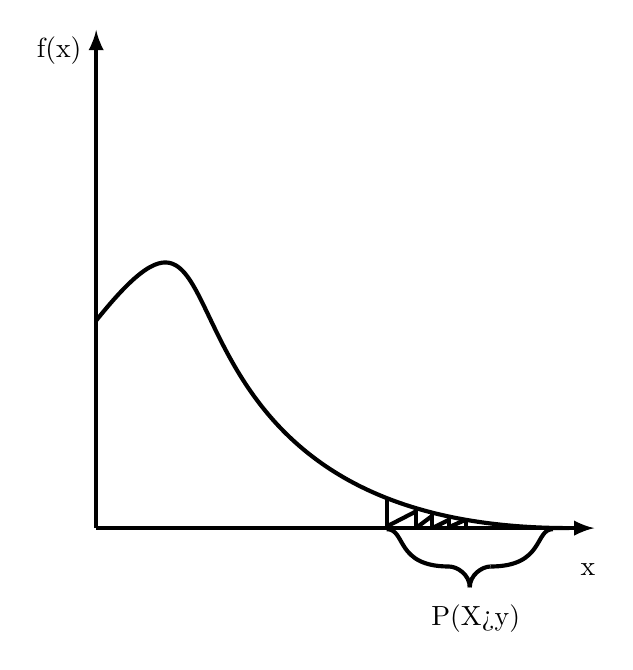
\begin{tikzpicture}
\pgftransformxscale{1.000000}
\pgftransformyscale{-1.000000}
\definecolor{dialinecolor}{rgb}{0.000000, 0.000000, 0.000000}
\pgfsetstrokecolor{dialinecolor}
\definecolor{dialinecolor}{rgb}{1.000000, 1.000000, 1.000000}
\pgfsetfillcolor{dialinecolor}
\pgfsetlinewidth{0.100000\du}
\pgfsetdash{}{0pt}
\pgfsetdash{}{0pt}
\pgfsetbuttcap
{
\definecolor{dialinecolor}{rgb}{0.000000, 0.000000, 0.000000}
\pgfsetfillcolor{dialinecolor}
% was here!!!
\pgfsetarrowsend{latex}
\definecolor{dialinecolor}{rgb}{0.000000, 0.000000, 0.000000}
\pgfsetstrokecolor{dialinecolor}
\draw (12.000000\du,0.000000\du)--(24.000000\du,0.000000\du);
}
\pgfsetlinewidth{0.100000\du}
\pgfsetdash{}{0pt}
\pgfsetdash{}{0pt}
\pgfsetbuttcap
{
\definecolor{dialinecolor}{rgb}{0.000000, 0.000000, 0.000000}
\pgfsetfillcolor{dialinecolor}
% was here!!!
\pgfsetarrowsend{latex}
\definecolor{dialinecolor}{rgb}{0.000000, 0.000000, 0.000000}
\pgfsetstrokecolor{dialinecolor}
\draw (12.000000\du,0.000000\du)--(12.000000\du,-12.000000\du);
}
\pgfsetlinewidth{0.100000\du}
\pgfsetdash{}{0pt}
\pgfsetdash{}{0pt}
\pgfsetmiterjoin
\pgfsetbuttcap
{
\definecolor{dialinecolor}{rgb}{0.000000, 0.000000, 0.000000}
\pgfsetfillcolor{dialinecolor}
% was here!!!
\definecolor{dialinecolor}{rgb}{0.000000, 0.000000, 0.000000}
\pgfsetstrokecolor{dialinecolor}
\pgfpathmoveto{\pgfpoint{23.400000\du}{0.000000\du}}
\pgfpathcurveto{\pgfpoint{12.400000\du}{0.000000\du}}{\pgfpoint{16.000000\du}{-10.000000\du}}{\pgfpoint{12.000000\du}{-5.000000\du}}
\pgfusepath{stroke}
}
\pgfsetlinewidth{0.100000\du}
\pgfsetdash{}{0pt}
\pgfsetdash{}{0pt}
\pgfsetbuttcap
{
\definecolor{dialinecolor}{rgb}{0.000000, 0.000000, 0.000000}
\pgfsetfillcolor{dialinecolor}
% was here!!!
\definecolor{dialinecolor}{rgb}{0.000000, 0.000000, 0.000000}
\pgfsetstrokecolor{dialinecolor}
\draw (19.000000\du,-0.700000\du)--(19.000000\du,0.000000\du);
}
\pgfsetlinewidth{0.100000\du}
\pgfsetdash{}{0pt}
\pgfsetdash{}{0pt}
\pgfsetmiterjoin
\pgfsetbuttcap
{
\definecolor{dialinecolor}{rgb}{0.000000, 0.000000, 0.000000}
\pgfsetfillcolor{dialinecolor}
% was here!!!
{\pgfsetcornersarced{\pgfpoint{0.000000\du}{0.000000\du}}\definecolor{dialinecolor}{rgb}{0.000000, 0.000000, 0.000000}
\pgfsetstrokecolor{dialinecolor}
\draw (19.032329\du,-0.056240\du)--(19.700000\du,-0.400000\du);
}}
\pgfsetlinewidth{0.100000\du}
\pgfsetdash{}{0pt}
\pgfsetdash{}{0pt}
\pgfsetmiterjoin
\pgfsetbuttcap
{
\definecolor{dialinecolor}{rgb}{0.000000, 0.000000, 0.000000}
\pgfsetfillcolor{dialinecolor}
% was here!!!
{\pgfsetcornersarced{\pgfpoint{0.000000\du}{0.000000\du}}\definecolor{dialinecolor}{rgb}{0.000000, 0.000000, 0.000000}
\pgfsetstrokecolor{dialinecolor}
\draw (19.700000\du,-0.500000\du)--(19.700000\du,0.000000\du);
}}
\pgfsetlinewidth{0.100000\du}
\pgfsetdash{}{0pt}
\pgfsetdash{}{0pt}
\pgfsetmiterjoin
\pgfsetbuttcap
{
\definecolor{dialinecolor}{rgb}{0.000000, 0.000000, 0.000000}
\pgfsetfillcolor{dialinecolor}
% was here!!!
{\pgfsetcornersarced{\pgfpoint{0.000000\du}{0.000000\du}}\definecolor{dialinecolor}{rgb}{0.000000, 0.000000, 0.000000}
\pgfsetstrokecolor{dialinecolor}
\draw (19.700000\du,0.000000\du)--(20.100000\du,-0.300000\du);
}}
\pgfsetlinewidth{0.100000\du}
\pgfsetdash{}{0pt}
\pgfsetdash{}{0pt}
\pgfsetbuttcap
{
\definecolor{dialinecolor}{rgb}{0.000000, 0.000000, 0.000000}
\pgfsetfillcolor{dialinecolor}
% was here!!!
\definecolor{dialinecolor}{rgb}{0.000000, 0.000000, 0.000000}
\pgfsetstrokecolor{dialinecolor}
\draw (20.100000\du,-0.400000\du)--(20.100000\du,0.000000\du);
}
\pgfsetlinewidth{0.100000\du}
\pgfsetdash{}{0pt}
\pgfsetdash{}{0pt}
\pgfsetmiterjoin
\pgfsetbuttcap
{
\definecolor{dialinecolor}{rgb}{0.000000, 0.000000, 0.000000}
\pgfsetfillcolor{dialinecolor}
% was here!!!
{\pgfsetcornersarced{\pgfpoint{0.000000\du}{0.000000\du}}\definecolor{dialinecolor}{rgb}{0.000000, 0.000000, 0.000000}
\pgfsetstrokecolor{dialinecolor}
\draw (20.100000\du,0.000000\du)--(20.500000\du,-0.200000\du);
}}
\pgfsetlinewidth{0.100000\du}
\pgfsetdash{}{0pt}
\pgfsetdash{}{0pt}
\pgfsetmiterjoin
\pgfsetbuttcap
{
\definecolor{dialinecolor}{rgb}{0.000000, 0.000000, 0.000000}
\pgfsetfillcolor{dialinecolor}
% was here!!!
{\pgfsetcornersarced{\pgfpoint{0.000000\du}{0.000000\du}}\definecolor{dialinecolor}{rgb}{0.000000, 0.000000, 0.000000}
\pgfsetstrokecolor{dialinecolor}
\draw (20.500000\du,-0.300000\du)--(20.500000\du,0.000000\du);
}}
\pgfsetlinewidth{0.100000\du}
\pgfsetdash{}{0pt}
\pgfsetdash{}{0pt}
\pgfsetmiterjoin
\pgfsetbuttcap
{
\definecolor{dialinecolor}{rgb}{0.000000, 0.000000, 0.000000}
\pgfsetfillcolor{dialinecolor}
% was here!!!
{\pgfsetcornersarced{\pgfpoint{0.000000\du}{0.000000\du}}\definecolor{dialinecolor}{rgb}{0.000000, 0.000000, 0.000000}
\pgfsetstrokecolor{dialinecolor}
\draw (20.900000\du,-0.200000\du)--(20.476079\du,-0.012490\du);
}}
\pgfsetlinewidth{0.100000\du}
\pgfsetdash{}{0pt}
\pgfsetdash{}{0pt}
\pgfsetmiterjoin
\pgfsetbuttcap
{
\definecolor{dialinecolor}{rgb}{0.000000, 0.000000, 0.000000}
\pgfsetfillcolor{dialinecolor}
% was here!!!
\definecolor{dialinecolor}{rgb}{0.000000, 0.000000, 0.000000}
\pgfsetstrokecolor{dialinecolor}
\pgfpathmoveto{\pgfpoint{19.000000\du}{0.025000\du}}
\pgfpathcurveto{\pgfpoint{19.468950\du}{0.025000\du}}{\pgfpoint{19.200000\du}{0.925000\du}}{\pgfpoint{20.500000\du}{0.925000\du}}
\pgfusepath{stroke}
}
\pgfsetlinewidth{0.100000\du}
\pgfsetdash{}{0pt}
\pgfsetdash{}{0pt}
\pgfsetmiterjoin
\pgfsetbuttcap
{
\definecolor{dialinecolor}{rgb}{0.000000, 0.000000, 0.000000}
\pgfsetfillcolor{dialinecolor}
% was here!!!
\definecolor{dialinecolor}{rgb}{0.000000, 0.000000, 0.000000}
\pgfsetstrokecolor{dialinecolor}
\pgfpathmoveto{\pgfpoint{21.500000\du}{0.925000\du}}
\pgfpathcurveto{\pgfpoint{22.800000\du}{0.925000\du}}{\pgfpoint{22.558025\du}{0.025000\du}}{\pgfpoint{23.000000\du}{0.025000\du}}
\pgfusepath{stroke}
}
\pgfsetlinewidth{0.100000\du}
\pgfsetdash{}{0pt}
\pgfsetdash{}{0pt}
\pgfsetmiterjoin
\pgfsetbuttcap
{
\definecolor{dialinecolor}{rgb}{0.000000, 0.000000, 0.000000}
\pgfsetfillcolor{dialinecolor}
% was here!!!
\definecolor{dialinecolor}{rgb}{0.000000, 0.000000, 0.000000}
\pgfsetstrokecolor{dialinecolor}
\pgfpathmoveto{\pgfpoint{20.500000\du}{0.925000\du}}
\pgfpathcurveto{\pgfpoint{20.700000\du}{0.925000\du}}{\pgfpoint{21.000000\du}{1.125000\du}}{\pgfpoint{21.000000\du}{1.425000\du}}
\pgfusepath{stroke}
}
\pgfsetlinewidth{0.100000\du}
\pgfsetdash{}{0pt}
\pgfsetdash{}{0pt}
\pgfsetmiterjoin
\pgfsetbuttcap
{
\definecolor{dialinecolor}{rgb}{0.000000, 0.000000, 0.000000}
\pgfsetfillcolor{dialinecolor}
% was here!!!
\definecolor{dialinecolor}{rgb}{0.000000, 0.000000, 0.000000}
\pgfsetstrokecolor{dialinecolor}
\pgfpathmoveto{\pgfpoint{21.500000\du}{0.925000\du}}
\pgfpathcurveto{\pgfpoint{21.300000\du}{0.925000\du}}{\pgfpoint{21.000000\du}{1.125000\du}}{\pgfpoint{21.000000\du}{1.425000\du}}
\pgfusepath{stroke}
}
% setfont left to latex
\definecolor{dialinecolor}{rgb}{0.000000, 0.000000, 0.000000}
\pgfsetstrokecolor{dialinecolor}
\node[anchor=west] at (19.800000\du,2.175000\du){P(X>y)};
% setfont left to latex
\definecolor{dialinecolor}{rgb}{0.000000, 0.000000, 0.000000}
\pgfsetstrokecolor{dialinecolor}
\node[anchor=west] at (10.300000\du,-11.500000\du){f(x)};
% setfont left to latex
\definecolor{dialinecolor}{rgb}{0.000000, 0.000000, 0.000000}
\pgfsetstrokecolor{dialinecolor}
\node[anchor=west] at (23.400000\du,1.000000\du){x};
% setfont left to latex
\definecolor{dialinecolor}{rgb}{0.000000, 0.000000, 0.000000}
\pgfsetstrokecolor{dialinecolor}
\node[anchor=west] at (22.000000\du,1.000000\du){};
\pgfsetlinewidth{0.100000\du}
\pgfsetdash{}{0pt}
\pgfsetdash{}{0pt}
\pgfsetbuttcap
{
\definecolor{dialinecolor}{rgb}{0.000000, 0.000000, 0.000000}
\pgfsetfillcolor{dialinecolor}
% was here!!!
\definecolor{dialinecolor}{rgb}{0.000000, 0.000000, 0.000000}
\pgfsetstrokecolor{dialinecolor}
\draw (20.900000\du,-0.200000\du)--(20.900000\du,0.000000\du);
}
\end{tikzpicture}

  \caption{Probabilité à l'extrémité du support}
  \label{fig:probdroite}
\end{figure}

C'est dans cette optique qu'ont été développées les approximations par
la méthode du point de selle. Puisque celle-ci requiert l'utilisation
de l'approximation de Laplace pour la fonction de densité et de
l'approximation de Temme pour la fonction de répartition, on les
introduit avant de développer la méthode à proprement parler. Il est à
noter que la majorité de ces démonstrations sont tirées de
\cite{butler2007saddlepoint} qui présente une monographie assez
complète sur la méthode du point de selle.

\section{L'approximation de Laplace}
\label{sec:appr-de-lapl}

L'approximation de Laplace sera utilisée afin de développer la méthode
du point de selle pour la fonction de densité.  Soit $g(x)$, une
fonction régulière sur l'intervalle $\left[c,d\right]$ ayant un
minimum global au point $\hat{x} \in
\left]c,d\right]$. L'approximation de Laplace de premier ordre prend
la forme suivante:
\begin{align}
  \label{eq:approxlaplace1}
  \int_{c}^{d} e^{-g(x)}dx &\approx
  \frac{\sqrt{2\pi}e^{-g(\hat{x})}}{\sqrt{g^{\prime\prime}(\hat{x})}}.
\end{align}

La démonstration se fait facilement en utilisant le développement de
Taylor de $g(x)$ autour du point $\hat{x}$:
\begin{align}
  \label{eq:taylorgx}
  g(x) &= g(\hat{x}) + g^{\prime}(\hat{x})(x-\hat{x}) + \frac{1}{2}
  g^{\prime\prime}(\hat{x})(x-\hat{x})^2 + R.
\end{align}

La valeur $R$ représente le reste du développement et est une quantité
relativement petite. Comme $\hat{x}$ est un minimum local, alors la
dérivée première $g^{\prime}(\hat{x})$ vaut $0$ et la dérivée seconde
$g^{\prime\prime}(\hat{x})$ est supérieure à 0. On obtient donc
l'intégrale suivante, qui ressemble à celle de la fonction de
répartition de la distribution normale:
\begin{align}
  \label{eq:integraleapproxlaplace1}
  e^{-g(\hat{x})}\int_{c}^{d}
  \exp{\left\{-\frac{1}{2}g^{\prime\prime}(\hat{x})(x-\hat{x})^2
    \right\}}dx &\approx e^{-g(\hat{x})}
  \sqrt{\frac{2\pi}{g^{\prime\prime}(\hat{x})}}.
\end{align}

En utilisant un terme de plus du développement de Taylor
\eqref{eq:taylorgx}, on obtient l'approximation de Laplace de second
ordre, qui a une plus grande précision:
\begin{align}
  \label{eq:approxlaplace2}
  \int_{c}^{d} e^{-g(x)}dx &\approx
  \frac{\sqrt{2\pi}e^{-g(\hat{x})}}{\sqrt{g^{\prime\prime}(\hat{x})}}\left\{\frac{5}{24}\hat{\kappa}_3^2
    - \frac{1}{8} \hat{\kappa}_4 \right\}
\end{align}

où
\begin{align}
  \hat{\kappa}_i &=
  \frac{g^{(i)}(\hat{x})}{\left\{g^{\prime\prime}(\hat{x})\right\}^{i/2}}
  ,\quad i\geq 3 \label{eq:kappailaplace}.
\end{align}

\section{L'approximation de Temme}
\label{sec:lappr-de-temme}

L'approximation de Temme sera utilisée afin de dériver la méthode du
point de selle pour la fonction de répartition.  On considère une
variable aléatoire $Z_{w_0}$ de distribution normale standard tronquée
de telle sorte qu'elle ne puisse prendre des valeurs supérieures au
point $w_0$.
\begin{figure}[!ht]
  \centering % Graphic for TeX using PGF
% Title: /home/francois/projet-de-maitrise/graphiques/normaletronque.dia
% Creator: Dia v0.97.2
% CreationDate: Tue Jul 30 16:24:46 2013
% For: francois
% \usepackage{tikz}
% The following commands are not supported in PSTricks at present
% We define them conditionally, so when they are implemented,
% this pgf file will use them.
\ifx\du\undefined
  \newlength{\du}
\fi
\setlength{\du}{15\unitlength}
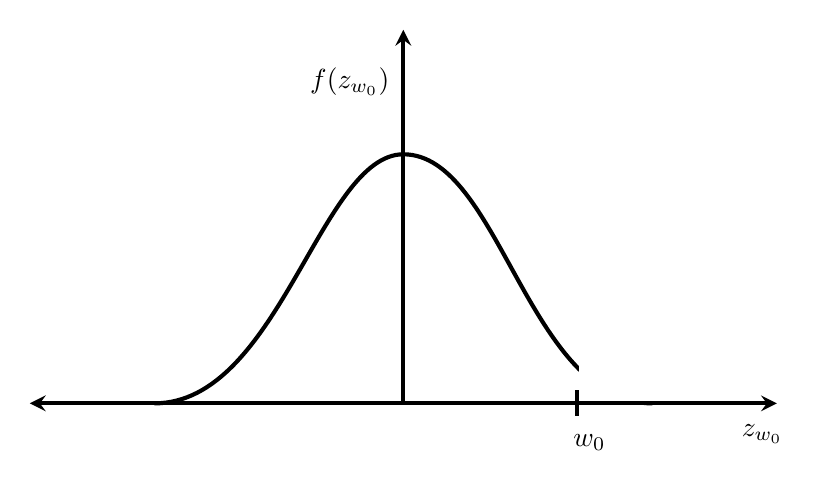
\begin{tikzpicture}
\pgftransformxscale{1.000000}
\pgftransformyscale{-1.000000}
\definecolor{dialinecolor}{rgb}{0.000000, 0.000000, 0.000000}
\pgfsetstrokecolor{dialinecolor}
\definecolor{dialinecolor}{rgb}{1.000000, 1.000000, 1.000000}
\pgfsetfillcolor{dialinecolor}
\pgfsetlinewidth{0.100000\du}
\pgfsetdash{}{0pt}
\pgfsetdash{}{0pt}
\pgfsetbuttcap
{
\definecolor{dialinecolor}{rgb}{0.000000, 0.000000, 0.000000}
\pgfsetfillcolor{dialinecolor}
% was here!!!
\pgfsetarrowsstart{stealth}
\pgfsetarrowsend{stealth}
\definecolor{dialinecolor}{rgb}{0.000000, 0.000000, 0.000000}
\pgfsetstrokecolor{dialinecolor}
\draw (18.000000\du,24.000000\du)--(36.000000\du,24.000000\du);
}
\pgfsetlinewidth{0.100000\du}
\pgfsetdash{}{0pt}
\pgfsetdash{}{0pt}
\pgfsetbuttcap
{
\definecolor{dialinecolor}{rgb}{0.000000, 0.000000, 0.000000}
\pgfsetfillcolor{dialinecolor}
% was here!!!
\pgfsetarrowsend{stealth}
\definecolor{dialinecolor}{rgb}{0.000000, 0.000000, 0.000000}
\pgfsetstrokecolor{dialinecolor}
\draw (27.000000\du,24.000000\du)--(27.000000\du,15.000000\du);
}
\pgfsetlinewidth{0.100000\du}
\pgfsetdash{}{0pt}
\pgfsetdash{}{0pt}
\pgfsetmiterjoin
\pgfsetbuttcap
{
\definecolor{dialinecolor}{rgb}{0.000000, 0.000000, 0.000000}
\pgfsetfillcolor{dialinecolor}
% was here!!!
\definecolor{dialinecolor}{rgb}{0.000000, 0.000000, 0.000000}
\pgfsetstrokecolor{dialinecolor}
\pgfpathmoveto{\pgfpoint{21.000000\du}{24.000000\du}}
\pgfpathcurveto{\pgfpoint{24.000000\du}{24.000000\du}}{\pgfpoint{25.008000\du}{18.000000\du}}{\pgfpoint{27.000000\du}{18.000000\du}}
\pgfusepath{stroke}
}
\pgfsetlinewidth{0.100000\du}
\pgfsetdash{}{0pt}
\pgfsetdash{}{0pt}
\pgfsetmiterjoin
\pgfsetbuttcap
{
\definecolor{dialinecolor}{rgb}{0.000000, 0.000000, 0.000000}
\pgfsetfillcolor{dialinecolor}
% was here!!!
\definecolor{dialinecolor}{rgb}{0.000000, 0.000000, 0.000000}
\pgfsetstrokecolor{dialinecolor}
\pgfpathmoveto{\pgfpoint{27.000000\du}{18.000000\du}}
\pgfpathcurveto{\pgfpoint{29.324000\du}{18.000000\du}}{\pgfpoint{30.000000\du}{24.000000\du}}{\pgfpoint{33.000000\du}{24.000000\du}}
\pgfusepath{stroke}
}
\pgfsetlinewidth{0.100000\du}
\pgfsetdash{}{0pt}
\pgfsetdash{}{0pt}
\pgfsetmiterjoin
\definecolor{dialinecolor}{rgb}{1.000000, 1.000000, 1.000000}
\pgfsetfillcolor{dialinecolor}
\fill (31.287500\du,22.975000\du)--(31.287500\du,23.900000\du)--(33.087500\du,23.900000\du)--(33.087500\du,22.975000\du)--cycle;
\definecolor{dialinecolor}{rgb}{1.000000, 1.000000, 1.000000}
\pgfsetstrokecolor{dialinecolor}
\draw (31.287500\du,22.975000\du)--(31.287500\du,23.900000\du)--(33.087500\du,23.900000\du)--(33.087500\du,22.975000\du)--cycle;
\pgfsetlinewidth{0.100000\du}
\pgfsetdash{}{0pt}
\pgfsetdash{}{0pt}
\pgfsetbuttcap
{
\definecolor{dialinecolor}{rgb}{0.000000, 0.000000, 0.000000}
\pgfsetfillcolor{dialinecolor}
% was here!!!
\definecolor{dialinecolor}{rgb}{0.000000, 0.000000, 0.000000}
\pgfsetstrokecolor{dialinecolor}
\draw (31.185444\du,23.681250\du)--(31.185444\du,24.312500\du);
}
% setfont left to latex
\definecolor{dialinecolor}{rgb}{0.000000, 0.000000, 0.000000}
\pgfsetstrokecolor{dialinecolor}
\node[anchor=west] at (30.821374\du,24.943750\du){$w_0$};
% setfont left to latex
\definecolor{dialinecolor}{rgb}{0.000000, 0.000000, 0.000000}
\pgfsetstrokecolor{dialinecolor}
\node[anchor=west] at (34.881350\du,24.743750\du){$z_{w_0}$};
% setfont left to latex
\definecolor{dialinecolor}{rgb}{0.000000, 0.000000, 0.000000}
\pgfsetstrokecolor{dialinecolor}
\node[anchor=west] at (24.484382\du,16.243750\du){$f(z_{w_0})$};
\end{tikzpicture}

  \caption{Distribution normale tronquée à $w_0$}
  \label{fig:normaletronque}
\end{figure}

On définit l'espérance d'une fonction $h$ de cette variable aléatoire, 
à partir des fonctions de densité $\phi(w)$ et de répartition
$\Phi(w)$ de la loi normale, comme suit:
\begin{align}
  E[h(Z_{w_0})] &= \frac{\int_{-\infty}^{w_0} h(w)\phi(w)
    dw}{\Phi(w_0)}.
\end{align}

Une approximation du numérateur est donnée par le développement
suivant:
\begin{align*}
  \int_{-\infty}^{w_0} h(w)\phi(w) dw &= h(0)\Phi(w_0)+\int_{-\infty}^{w_0} \frac{h(w)-h(0)}{w} w\phi(w)dw \nonumber\\
  &= h(0)\Phi(w_0)-\int_{-\infty}^{w_0} \frac{h(w)-h(0)}{w} d\phi(w)\quad \mbox{(car }w\phi(w)dw = -d\phi(w) \mbox{)} \nonumber\\
  &\approx h(0)\Phi(w_0) - \left[ \frac{h(w)-h(0)}{w} \phi(w) \right]_{w=-\infty}^{w=w_0}. \nonumber\\
\end{align*}

On ignore l'intégrale de l'intégration par parties, puisqu'elle prend
une petite valeur, pour obtenir l'approximation de Temme :
\begin{align}
  \label{eq:temmeintegrale}
  \int_{-\infty}^{w_0} h(w)\phi(w) dw &\approx h(0)\Phi(w_0) +
  \phi(w_0) \left[ \frac{h(w_0)-h(0)}{w_0} \right].
\end{align}

\section{La méthode du point de selle}
\label{sec:pointcolGAL}

L'approximation de la distribution d'une variable aléatoire par la
méthode du point de selle a été introduite par
\cite{daniels1954saddlepoint}. Il cherchait une façon d'estimer la
distribution de la moyenne de variables aléatoires.

\subsection{Approximation de la densité}
\label{sec:appr-de-prem}

Soit une variable aléatoire $Y$ dont on cherche à évaluer la fonction
de densité $f_Y(y)$. Les fonctions génératrices des moments $M_Y( s)$
et des cumulants $K_Y( s)$ sont définies de manière équivalente par
les intégrales suivantes, où l'on cherche une forme qui permettra
d'utiliser l'approximation de Laplace:
\begin{align}
  M_Y( s) = e^{K_Y( s)} &= \int_{-\infty}^{\infty} e^{ s y} f_Y(y) dy \label{eq:FGMdefinitionsaddle}\\
  &= \int_{-\infty}^{\infty} e^{ s y + \ln{f_Y(y)}} dy \label{eq:FGMdaniels}\\
  &= \int_{-\infty}^{\infty} e^{-g( s,y)} dy.
\end{align}

Cette intégrale doit converger pour toute valeur $s$ comprise dans un
intervalle $\left]-c_1,c_2\right[$ contenant l'origine et où la somme
des bornes est positive: $c_1+c_2 > 0$. Cet intervalle doit être
choisi de sorte qu'il soit le plus grand possible. On considère pour
l'instant que la fonction $g( s,y) = - s y - \ln{f_Y(y)}$ répond aux
conditions de l'approximation de Laplace énoncées au début de la
section \ref{sec:appr-de-lapl}. On obtient alors l'approximation
suivante pour une valeur de $s$ fixée:
\begin{align}
  \label{eq:laplacesaddle1}
  e^{K(s)} &\approx \sqrt{\frac{2\pi}{g^{\prime\prime}( s,\hat{y}_{
        s})}}e^{ s \hat{y}_{ s}} f_Y(\hat{y}_{ s}).
\end{align}

La valeur $\hat{y}_{s}$ est celle qui minimise la fonction $g(s,y)$
pour un point $s$ fixé. C'est donc la solution de la condition de
premier ordre:
\begin{align}
  0 &= -g^{\prime}( s,\hat{y}_{ s}) \nonumber\\
  &=  s + \frac{\partial \ln{(f_Y(\hat{y}_{ s})}}{\partial \hat{y}_{ s}} \nonumber\\
  s &= - \frac{\partial \ln{(f_Y(\hat{y}_{ s})}}{\partial \hat{y}_{
      s}}. \label{eq:premierordresaddle}
\end{align}

L'hypothèse posée afin de faire l'approximation est que la fonction
$g(s)$ est convexe, ce qui implique que la dérivée seconde de celle-ci
est positive $(\frac{\partial^2g( s,y)}{\partial y^2} > 0)$ par
définition. On examine la relation entre le point de selle $s$ et le
point $\hat{y}_{ s}$ déterminé par l'équation
\eqref{eq:premierordresaddle}. En dérivant celle-ci par rapport au
point $\hat{y}_{ s}$, on constate qu'il existe une relation croissante
et monotone entre les deux:
\begin{align}
  \label{eq:secondordresaddle}
  \frac{d s}{d\hat{y}_{ s}} &= - \frac{\partial^2 \ln{(f_Y(\hat{y}_{
        s})}}{\partial \hat{y}_{ s}^2} > 0.
\end{align}

On doit maintenant trouver une solution de l'équation de premier ordre
\eqref{eq:premierordresaddle}. Pour ce faire, on isole le terme
$\ln{f_Y(y)}$ dans l'équation \eqref{eq:laplacesaddle1}:
\begin{align}
  \label{eq:lnfysaddlelaplace}
  \ln{f_Y(y)} & \approx K( s) - s \hat{y}_{ s} - \frac{1}{2}
  \ln{\left(\frac{2\pi}{-\left(\frac{\partial^2 \ln{(f_Y(\hat{y}_{
                s}))}}{\partial \hat{y}_{ s}^2}\right)}\right)}.
\end{align}

Si l'on considère que le dernier terme de la soustraction est
relativement constant par rapport au point $\hat{y}_{ s}$, alors sa
dérivée sera pratiquement nulle. Ce terme peut donc être négligé dans
la prochaine étape, où on dérive \eqref{eq:lnfysaddlelaplace} par
rapport à $y_s$:
\begin{align}
  \frac{\partial \ln{f_Y(\hat{y}_{s})}}{\partial \hat{y}_{s}}
  &\approx \left(K^{\prime}(s) - \hat{y}_{s}\right)\frac{\partial
    s}{\partial
    \hat{y}_{s} } -  s.\label{eq:dlnfysaddlelaplace}
\end{align}

En combinant l'approximation \eqref{eq:dlnfysaddlelaplace} et la
condition de premier ordre \eqref{eq:premierordresaddle}, il en
résulte que le terme de gauche de la partie de droite est
approximativement égal à 0:
\begin{align}
  \label{eq:premierodreapprox}
  \left(K^{\prime}( s) - \hat{y}_{ s}\right)\frac{\partial s}{\partial
    \hat{y}_{s} } &\approx 0.
\end{align}

Cela conduit donc à l'équation qui met en relation le point de
selle $s$ et le point $\hat{y}_{ s}$:
\begin{align}
  \label{eq:saddlepoint}
  \hat{y}_{ s} &= K^{\prime}(s).
\end{align}

Enfin, la dernière relation consiste à exprimer $g^{\prime\prime}(
s,\hat{y}_{ s})$ seulement en fonction du point de selle $s$ en
utilisant la condition de second ordre \eqref{eq:secondordresaddle} et
en dérivant l'équation précédente \eqref{eq:saddlepoint} en $s$:
\begin{align}
  \label{eq:deriveesecondesaddlepoint}
  g^{\prime\prime}( s,\hat{y}_{ s}) &= - \frac{\partial^2
    \ln{(f_Y(\hat{y_{s}}))}}{\partial \hat{y}_{ s}^2} \nonumber\\
  &= \frac{d  s}{d\hat{y}_{ s}} \nonumber\\
  &= \left(\frac{d\hat{y}_{ s}}{d  s}\right)^{-1} \nonumber\\
  &= \left(K^{\prime\prime}( s)\right)^{-1}.
\end{align}

On peut donc réécrire l'approximation de Laplace
\eqref{eq:laplacesaddle1} en utilisant les relations
\eqref{eq:saddlepoint} et \eqref{eq:deriveesecondesaddlepoint}:
\begin{align}
  e^{K( s)} &\approx \sqrt{2\pi K^{\prime\prime}( s)}\exp{\left\{ s
      \hat{y}_{ s}\right\}}
  f_Y(\hat{y_{s}}) \nonumber\\
  \hat{f_Y}(y_{s}) &\approx \frac{1}{\sqrt{2\pi K^{\prime\prime}(
      \hat{s})}} \exp{\left\{K(\hat{s}) - \hat{s} y\right\}} =
  \hat{f}_Y(y).\label{eq:approximationsaddlepointordre1}
\end{align}

L'équation \eqref{eq:approximationsaddlepointordre1} est une
approximation par la méthode du point de selle de la densité de la
variable aléatoire $Y$ au point $y_{s}$.

Par convention, on considère que l'approximation $\hat{f}_Y(y)$ est
une fonction de densité, mais, elle n'en est pas exactement une
puisqu'elle n'intègre pas à 1. Cependant, il est possible de la
normaliser en calculant la valeur de l'intégrale de celle-ci sur le
domaine $\chi$ de la distribution, puis en divisant l'approximation
$\hat{f}_Y(y)$ par celle-ci:
\begin{subequations}\label{eq:normalisationsaddle}
  \begin{align}
    c &= \int_{\chi} \hat{f}_Y(y) dy \neq 1 \label{eq:normalisationsaddle1}\\
    \overline{f}_Y(y) &= c^{-1} \hat{f}_Y(y),\quad \forall y \in
    \chi. \label{eq:normalisationsaddle2}
  \end{align}
\end{subequations}

\subsection{Unicité du point de selle}
\label{sec:unicite-du-point}

\cite{daniels1954saddlepoint} démontre que l'équation du point de
selle \eqref{eq:saddlepoint} a une solution unique dans l'intervalle
$\left[-c_1,c_2 \right]$ sélectionné précédemment lorsque $y_0$ est
situé dans un intervalle $\left[a,b\right]$.

Pour ce faire, il présente une condition essentielle. Les limites
inférieure et supérieure de la dérivée première de la fonction
génératrice des cumulants doivent correspondre aux points $a$ et $b$
respectivement \eqref{eq:limitesderiveeK}:
\begin{align}
  \label{eq:limitesderiveeK}
  \lim_{s\to c_2} K'(s) = b \\
  \lim_{s\to -c_1} K'(s) = a.
\end{align}

On définit la fonction génératrice des moments de la différence entre
la variable aléatoire $Y$ et le point $y_0$ par $M(s,y)$.

Quand $a < y_0 < b$, la dérivée première prend la forme suivante:
\begin{align}
  \label{eq:6}
  M'(s,y_0) = \int_{a}^{b} (y-y_0) e^{s(y-y_0)} dF(y).
\end{align}

Les limites inférieure et supérieure de la fonction $M'(s,y_0)$ sont
respectivement $M'(-\infty,y_0) = -\infty$ et $M'(\infty,y_0) =
\infty$. De plus, la dérivée de celle-ci est toujours positive
$M''(s,y_0)>0$. Donc, pour chaque valeur $a < y_0 < b$, une racine
unique $\hat{s}$ de l'équation $M'(s,y_0)=0$ existe
nécessairement. Par conséquent, l'équation du point de selle
\eqref{eq:saddlepoint}, qui lui est équivalente, a aussi une solution
réelle unique.

% \subsection{Approximation de second ordre de la densité}
% \label{sec:appr-de-second}

% On reprend la définition de la fonction génératrice des moments
% \eqref{eq:FGMdefinitionsaddle}. En réorganisant les termes, on définit
% une fonction de densité décalée pour chaque valeur $ s \in
% \left]a,b\right[$:
% \begin{align}
%   \label{eq:nouvelledensiteordre2}
%   f_Y(y; s) = \exp{\left\{ s y - K( s)\right\}} f_Y(y)
% \end{align}

% Cet ensemble est défini comme étant la famille de densités décalées
% par rapport au point de selle $s$, et a été développé par
% Esscher. Soit $Y_{ s}$ la variable aléatoire ayant cette densité, dont
% la moyenne et la variance sont définies comme suit:
% \begin{align}
%   E[Y_{ s}] &= K^{\prime}( s) \label{eq:moyennetilted}\\
%   Var[Y_{ s}] &= K^{\prime\prime}( s) \label{eq:vartilted}
% \end{align}

% On remarque que lorsque l'on situe le point de selle à l'origine
% $(s=0)$, on retrouve la définition usuelle des deux premiers
% cumulants. On définit les cumulants standardisés de la variable
% aléatoire $Y_{ s}$, qui sont basés sur les coefficients de
% l'approximation de Laplace du second ordre \eqref{eq:kappailaplace}.
% \begin{align}
%   \hat{\kappa}_i &=
%   \frac{K^{(i)}(\hat{x})}{\left\{K^{\prime\prime}(\hat{x})\right\}^{i/2}}
%   ,\quad i\geq 3 \label{eq:kappaitilting}
% \end{align}

% On définit l'expansion d'Edgeworth d'ordre 2
% \nocite{abramowitz1965handbook} autour de la moyenne comme étant
% l'approximation suivante, basée sur la distribution normale
% $\mathcal{N}(\mu,\sigma^2)$:
% \begin{align}
%   \label{eq:edgeworthmoyenne}
%   f_Y(\mu) &\approx
%   \frac{1}{\sigma\sqrt{2\pi}}\left(1+\frac{1}{8}\kappa_4 -
%     \frac{5}{24} \kappa_3^2 \right)
% \end{align}

% La technique développée par Esscher utilise indirectement cette
% expansion. Elle consiste en deux étapes:
% \begin{enumerate}
% \item Représenter la fonction de densité de la variable aléatoire $Y$
%   en l'isolant dans l'expression \eqref{eq:nouvelledensiteordre2}:
%   \begin{align}
%     \label{eq:etape1esscher}
%     f_Y(y) = \exp{\left\{K( s)- s y \right\}} f_Y(y; s)
%   \end{align}
% \item Utiliser l'expansion \eqref{eq:edgeworthmoyenne} de la densité
%   $f_Y(y; s)$ autour d'un point $ s $ optimal, qui se trouve à être la
%   moyenne de la variable $Y_{ s}$ définie par
%   \eqref{eq:moyennetilted}, ce qui revient à résoudre l'équation du
%   point de selle \eqref{eq:saddlepoint} en $s$:
%   \begin{align*}
%     E[Y_{\hat{s}}] &= K^{\prime}(\hat{s}) = y
%   \end{align*}
% \end{enumerate}

% L'expansion prend donc la forme suivante en remplaçant l'écart-type
% $\sigma$ par la variance de la variable aléatoire $Y_{ s}$, exprimée à
% l'aide de la fonction génératrice des cumulants \eqref{eq:vartilted}.
% \begin{align}
%   \label{eq:edgeworthordre2}
%   f_Y(y;\hat{s}) &\approx \frac{1}{\sqrt{2\pi
%       K^{\prime\prime}(\hat{s})}} \left(1+\frac{1}{8}\kappa_4(\hat{s})
%     - \frac{5}{24} \kappa_3^2(\hat{s}) \right)
% \end{align}
% En substituant l'expansion \eqref{eq:edgeworthordre2} dans l'équation
% \eqref{eq:etape1esscher}, on obtient l'approximation par la méthode du
% point de selle d'ordre 2 de la densité de la variable aléatoire $Y$.
% \begin{align}
%   \label{eq:approximationsaddlepointordre2}
%   f_Y(y) &\approx \frac{1}{\sqrt{2\pi K^{\prime\prime}(\hat{s})}}
%   \exp{\left\{K(\hat{s})-\hat{s} y \right\}}
%   \left(1+\frac{1}{8}\kappa_4(\hat{s}) - \frac{5}{24}
%     \kappa_3^2(\hat{s}) \right)
% \end{align}

\subsection{Approximation de la fonction de
  répartition}
\label{sec:appr-de-prem-1}

La fonction de répartition de la variable aléatoire $Y$ au point $y$
est définie comme étant la probabilité $P(y \leq Y)$ et s'obtient en
intégrant la densité sur l'intervalle $\left[ -\infty,y \right]$. On
considère le changement de variable $y \mapsto \hat{w}$ défini comme
suit:
\begin{align}
  \label{eq:chengementytow}
  \frac{\hat{w}^2}{2} = \hat{s} y - K(\hat{s}).
\end{align}

La valeur $\hat{w}_y$ est obtenue en résolvant l'équation du point de
selle pour la racine $\hat{s}$ et en remplaçant celle-ci dans
l'équation \eqref{eq:chengementytow}.  Ce changement de variable est
une transformation monotone, continue et croissante dont la dérivée
est donnée par l'équation suivante:
\begin{align}
  \label{eq:derivchengementytow}
  \frac{dy}{d\hat{w}} = \begin{cases}
    \hat{w} / \hat{s}, & \hat{s} \neq 0 \\
    \sqrt{K^{\prime\prime}(0)}, & \hat{s} = 0.
  \end{cases}
\end{align}

L'approximation de premier ordre de la fonction de répartition
s'obtient en intégrant celle de premier ordre de la densité
\eqref{eq:approximationsaddlepointordre1} sur ce même intervalle à
l'aide du changement de variable \eqref{eq:chengementytow}:
\begin{align}
  \label{eq:approxintegraleREPordre1}
  F_Y(y) &\approx \int_{-\infty}^{y} \frac{1}{\sqrt{2\pi
      K^{\prime\prime}( s)}}
  \exp{\left\{K( s) -  s x\right\}} dx \nonumber\\
  &= \int_{-\infty}^{y} \frac{1}{\sqrt{K^{\prime\prime}( s)}}
  \phi(\hat{w}) dx \nonumber\\
  &= \int_{-\infty}^{\hat{w}_y}
  \frac{\hat{w}}{\hat{s}\sqrt{K^{\prime\prime}( s)}}\phi(\hat{w})
  d\hat{w}.
\end{align}

On applique l'approximation de Temme à l'intégrale précédente avec
l'équation:
\begin{align*}
  h(\hat{w})=\frac{\hat{w}}{\hat{s}\sqrt{K^{\prime\prime}( s)}}.
\end{align*}

On obtient ainsi l'approximation de premier ordre de la fonction de
répartition:
\begin{align}
  \label{eq:approximationsaddlepointREPordre1}
  F_Y(y) &\approx \Phi(\hat{w}_y) +
  \phi(\hat{w}_y)\frac{1-h(\hat{w}_y)}{\hat{w}_y} \nonumber\\
  & \approx \Phi(\hat{w}_y) + \phi(\hat{w}_y)
  \left(\frac{1}{\hat{w}_y}-\frac{1}{\hat{u}_y} \right).
\end{align}

Les deux constantes $\hat{w}_y$ et $\hat{u}_y$ sont respectivement
définies comme suit:
\begin{subequations}\label{eq:wuysaddlerepart2}
  \begin{align}
    \hat{w}_y &= \sgn(\hat{s})\sqrt{2\left\{\hat{s} y - K(\hat{s})\right\}} \label{eq:wysaddlerepart2}\\
    \hat{u}_y &=
    \hat{s}\sqrt{K^{\prime\prime}(\hat{s})} \label{eq:uysaddlerepart2}.
  \end{align}
\end{subequations}

% \subsection{Approximation de second ordre de la fonction de
%   répartition}
% \label{sec:appr-de-second-1}

% On reprend le développement précédent
% \eqref{eq:approxintegraleREPordre1}, mais avec l'approximation de
% second ordre de la densité \eqref{eq:approximationsaddlepointordre2}
% \citep{daniels1987tail}.
% \begin{align}
%   \label{eq:approxintegraleREPordre2}
%   F_Y(y) &\approx \int_{-\infty}^{y} \frac{\exp{\left\{K( s) - s
%         x\right\}}}{\sqrt{2\pi K^{\prime\prime}( s)}}
%   \left(1+\frac{1}{8}\kappa_4(\hat{s}) - \frac{5}{24}
%     \kappa_3^2(\hat{s}) \right) dx \nonumber\\
%   &= \int_{-\infty}^{\hat{w}_y}
%   \frac{\hat{w}}{\hat{s}\sqrt{K^{\prime\prime}(
%       s)}}\left(1+\frac{1}{8}\kappa_4(\hat{s}) - \frac{5}{24}
%     \kappa_3^2(\hat{s}) \right)\phi(\hat{w}) d\hat{w}
% \end{align}

% La fonction à utiliser pour l'approximation de Temme est alors
% \begin{align*}
%   h(\hat{w})=\frac{\hat{w}}{\hat{s}\sqrt{K^{\prime\prime}(
%       s)}}\left(1+\frac{1}{8}\kappa_4(\hat{s}) - \frac{5}{24}
%     \kappa_3^2(\hat{s}) \right)\phi(\hat{w})
% \end{align*}

% Ainsi, on obtient l'approximation de second ordre de la fonction de
% répartition.
% \begin{align}
%   \label{eq:approximationsaddlepointREPordre2}
%   F_Y(y) & \approx \Phi(\hat{w}_y) + \phi(\hat{w}_y)
%   \left(\frac{1}{\hat{w}_y}-\frac{1}{\hat{u}_y}(1-\frac{1}{8}
%     \hat{\kappa}_4+\frac{5}{24}\hat{\kappa}_3^2) \right)
% \end{align}

\subsection{Quelques propriétés des approximations}
\label{sec:proprietesaddle}

Les approximations par la méthode du point de selle ont pour
principale propriété de respecter le principe d'invariance. Cette
propriété permet notamment d'obtenir une approximation de la densité
ainsi que la fonction de répartition en utilisant des paramètres
estimés à partir d'un échantillon de données centrées et
réduites. Puis, elle permet d'appliquer la transformation
linéaire $Y = \sigma{X}+\mu$, telle qu'utilisée à la section
\ref{sec:transGAL}, tout en conservant la même approximation.

Une autre propriété de ces approximations est qu'elle respecte la
symétrie de la distribution. Ainsi, lorsque la distribution est
asymétrique, on doit s'attendre à ce que l'approximation le soit
aussi.

\section{Application de la méthode du point de selle}

\subsection{Approximation de la densité}
\label{sec:applicationsaddleGAL}

On applique la méthode du point de selle à la distribution de Laplace
asymétrique généralisée, afin d'obtenir une approximation de la
densité \eqref{eq:densitekotz} et aussi pouvoir représenter la
fonction de répartition, car la première n'est pas intégrable
analytiquement. Cependant, pour des fins de simplification, la
paramétrisation $\mu$ sera utilisée. On rappelle qu'on peut passer
d'une forme à l'autre à l'aide des équations \eqref{eq:mukappa} et
\eqref{eq:kappamu}.

On évalue d'abord la dérivée première de la fonction génératrice des
cumulants \eqref{eq:fgcGAL} par rapport à la variable de
transformation $s$:
\begin{align}
  \label{eq:derivcumulantGAL1}
  K^{\prime}_Y({s}) &=
  \frac{\partial}{\partial{s}}\ln\left(\frac{e^{\theta
        {s}}}{\left(1-\frac{1}{2} \sigma^2 {s}^2 - \mu {s}
      \right)^{\tau}}\right) \nonumber\\
  &= \frac{{\sigma}^{2}\theta{{s}}^{2}+\left(
      2\mu\theta-2{\sigma}^{2}\tau\right)
    {s}-2\theta-2\mu\tau}{{\sigma}^{2}{{s}}^{2}+2\mu{s}-2}, \\ & \quad
  \mbox{où } 1-\frac{1}{2} \sigma^2 {s}^2 - \mu {s} > 0.
\end{align}

On détermine ensuite le point de selle $\hat{s}_y$ correspondant à la
valeur $y$ pour laquelle on veut estimer la fonction de densité ou de
répartition, à l'aide de l'équation \eqref{eq:saddlepoint} et de la
première dérivée de la fonction génératrice des cumulants
\eqref{eq:derivcumulantGAL1}:
\begin{align*}
  y &= K^{\prime}_Y({\hat{s}_y}) \\
  &= \frac{{\sigma}^{2}\theta{\hat{s}_y}^{2}+\left(
      2\mu\theta-2{\sigma}^{2}\tau\right)
    {\hat{s}_y}-2\theta-2\mu\tau}{{\sigma}^{2}{{\hat{s}_y}}^{2}+2\mu{\hat{s}_y}-2}.
\end{align*}

L'équation précédente a deux solutions dont une seule correspond à un
minimum. Pour déterminer quelle solution est appropriée, on doit
évaluer la dérivée seconde en ces deux points:
\begin{align}
  \label{eq:saddlepointGAL}
  \hat{s}_y &=
  \frac{\pm\sqrt{2{\sigma}^{2}{{y}}^{2}+{\mu}^{2}{{y}}^{2}-4{\sigma}^{2}\theta{y}-2{\mu}^{2}\theta{y}+2{\sigma}^{2}{\theta}^{2}+{\mu}^{2}{\theta}^{2}+{\sigma}^{4}{\tau}^{2}}}{{\sigma}^{2}(y-\theta)}
  -\frac{\mu}{\sigma^{2}} -\frac{\tau}{y-\theta}.
\end{align}

On évalue la dérivée seconde de la fonction génératrice des cumulants:
\begin{align}
  \label{eq:derivcumulantGAL2}
  K^{\prime\prime}_Y({s}) &= \frac{2\left(
      {s}^{2}{\sigma}^{4}+2\mu{s}{\sigma}^{2}+2{\sigma}^{2}+2{\mu}^{2}\right)
    \tau}{{\left( {s}^{2}{\sigma}^{2}+2\mu{s}-2\right) }^{2}} > 0.
\end{align}

On peut maintenant déterminer quelle valeur $\hat{s}_y$ utiliser, car
la fonction $K^{\prime\prime}_Y({s})$ sera positive pour celle-ci. De manière équivalente, on utilise la condition
\ref{eq:fgmGALcond}, qui permet l'existence de la fonction génératrice
des moments, afin d'identifier plus aisément la solution unique.

On peut maintenant évaluer \eqref{eq:approximationsaddlepointordre1},
pour obtenir l'approximation de premier ordre de la fonction de
densité de la distribution de Laplace asymétrique généralisée.

% \subsection{Approximation de second ordre de la densité}

% L'évaluation de l'approximation de second ordre nécessite les
% dérivées troisième et quatrième de la fonction génératrice des
% cumulants:
% \begin{align}
%   \label{eq:K3K4GAL}
%   K^{\prime\prime\prime}({s}) &= -\frac{4\tau\left( {\sigma}^{2}{s}+\mu\right) \left( {\sigma}^{4}{{s}}^{2}+2\mu{\sigma}^{2}{s}+6{\sigma}^{2}+4{\mu}^{2}\right) }{{\left( {\sigma}^{2}{{s}}^{2}+2\mu{s}-2\right) }^{3}} \\
%   K^{iv}({s}) &= \frac{12\tau\left(
%     {\sigma}^{8}{s}^{4}+4\mu{\sigma}^{6}{s}^{3}+12{\sigma}^{6}{s}^{2}+12{\mu}^{2}{\sigma}^{4}{s}^{2}+24\mu{\sigma}^{4}{s}+16{\mu}^{3}{\sigma}^{2}{s}+4{\sigma}^{4}+16{\mu}^{2}{\sigma}^{2}+8{\mu}^{4}\right)
% }{{\left( {\sigma}^{2}{s}^{2}+2\mu{s}-2\right) }^{4}}
% \end{align}

% On peut ainsi évaluer les cumulants normalisés $\kappa_3(s)$ et
% $\kappa_4(s)$ à l'aide de la définition \eqref{eq:kappaitilting}.
% \begin{align}
%   \kappa_3(s) &= -\frac{\sqrt{2}\left( s{\sigma}^{2}+\mu\right) \left( {s}^{2}{\sigma}^{4}+2\mu{s}{\sigma}^{2}+6{\sigma}^{2}+4{\mu}^{2}\right) \left| {s}^{2}{\sigma}^{2}+2\mu{s}-2\right| \tau}{\left( {s}^{2}{\sigma}^{2}+2\mu{s}-2\right) {\left( \left( {s}^{2}{\sigma}^{4}+2\mu{s}{\sigma}^{2}+2{\sigma}^{2}+2{\mu}^{2}\right) \tau\right) }^{\frac{3}{2}}} \label{eq:kappa3gal}\\
%   \kappa_4(s) &= \frac{3\left(
%     {s}^{4}{\sigma}^{8}+4\mu{s}^{3}{\sigma}^{6}+12{s}^{2}{\sigma}^{6}+12{\mu}^{2}{s}^{2}{\sigma}^{4}+24\mu{s}{\sigma}^{4}+4{\sigma}^{4}+16{\mu}^{3}{s}{\sigma}^{2}+16{\mu}^{2}{\sigma}^{2}+8{\mu}^{4}\right)
% }{{\left(
%     {s}^{2}{\sigma}^{4}+2\mu{s}{\sigma}^{2}+2{\sigma}^{2}+2{\mu}^{2}\right)
% }^{2}\tau} \label{eq:kappa4gal}
% \end{align}

% En remplaçant ces valeurs dans l'équation
% \eqref{eq:approximationsaddlepointordre2}, on obtient
% l'approximation de second ordre de la densité de la distribution de
% Laplace asymétrique généralisée.

\subsection{Approximation de la fonction de répartition}

En évaluant les valeurs $\hat{w}_y \mbox{ et } \hat{u}_y$
\eqref{eq:wuysaddlerepart2} à l'aide de celles du point de selle
\eqref{eq:saddlepointGAL}, de la fonction génératrice des cumulants
\eqref{eq:fgcGAL} et de la dérivée seconde de cette dernière
\eqref{eq:derivcumulantGAL2}, on obtient l'approximation de premier
ordre de la fonction de répartition.

% Pour évaluer l'approximation de second ordre de la fonction de
% répartition \eqref{eq:approximationsaddlepointREPordre2}, on reprend
% les cumulants normalisés $\kappa_3(s) \text{ et } \kappa_4(s)$
% \eqref{eq:kappa3gal} \eqref{eq:kappa4gal} et on les remplace dans
% l'expression \eqref{eq:approximationsaddlepointREPordre2}.

Tout au long de ce chapitre, on a supposé que les paramètres de la
distribution étaient connus. Cependant, ceux-ci doivent être estimés à
partir des données d'un échantillon représentatif de la population
étudiée. C'est d'ailleurs ce qui sera fait dans les chapitres
suivants.

%%% Local Variables: 
%%% mode: latex
%%% TeX-master: "gabarit-maitrise"
%%% End: 
